\documentclass[twoside,a4paper]{article}
\usepackage{geometry}
\geometry{margin=1.5cm, vmargin={0pt,1cm}}
\setlength{\topmargin}{-1cm}
\setlength{\paperheight}{29.7cm}
\setlength{\textheight}{25.3cm}

% useful packages.
\usepackage{amsfonts}
\usepackage{amsmath}
\usepackage{amssymb}
\usepackage{amsthm}
\usepackage{enumerate}
\usepackage{graphicx}
\usepackage{multicol}
\usepackage{fancyhdr}
\usepackage{layout}

% some common command
\newcommand{\dif}{\mathrm{d}}
\newcommand{\avg}[1]{\left\langle #1 \right\rangle}
\newcommand{\difFrac}[2]{\frac{\dif #1}{\dif #2}}
\newcommand{\pdfFrac}[2]{\frac{\partial #1}{\partial #2}}
\newcommand{\OFL}{\mathrm{OFL}}
\newcommand{\UFL}{\mathrm{UFL}}
\newcommand{\fl}{\mathrm{fl}}
\newcommand{\op}{\odot}
\newcommand{\Eabs}{E_{\mathrm{abs}}}
\newcommand{\Erel}{E_{\mathrm{rel}}}

\begin{document}

\pagestyle{fancy}
\fancyhead{}
\lhead{Jovi Wong (3180104829)}
\chead{Numerical Analysis homework \#05}
\rhead{2020/4/17}


\section*{I. Scaled Integral of B-splines}
By theorem 4.25, we have
\begin{gather}
\frac{(n+1)B_i^n(x)}{t_{i+n}-t_{i-1}}=\dif B_i^{n+1}(x) + \frac{(n+1)B_{i+1}^n(x)}{t_{i+n+1}-t_i}\dif x\\
\frac{(n+1)B_{i+1}^n(x)}{t_{i+n+1}-t_{i}}=\dif B_{i+1}^{n+1}(x) + \frac{(n+1)B_{i+2}^n(x)}{t_{i+n+2}-t_{i+1}}\dif x\\
\cdots\\
\frac{(n+1)B_{i+n}^n(x)}{t_{i+2n}-t_{i+n-1}}=\dif B_{i+n}^{n+1}(x) + \frac{(n+1)B_{i+n+1}^n(x)}{t_{i+2n+1}-t_{i+n}}\dif x
\end{gather}
So add up LHS and RHS together, we can get 
\[
\frac{(n+1)B_i^n(x)}{t_{i+n}-t_{i-1}}=\sum_{k=0}^n \dif B_{i+k}^{n+1}(x) + \frac{(n+1)B_{i+n+1}^n(x)}{t_{i+2n+1}-t_{i+n}} \dif x
\]
Then apply $\int_{t_{i-1}}^{t_{i+n}}$ to both sides, 
\begin{gather}
\int_{t_{i-1}}^{t_{i+n}}\frac{(n+1)B_i^n(x)}{t_{i+n}-t_{i-1}}=\sum_{k=0}^n \int_{t_{i-1}}^{t_{i+n}}\dif B_{i+k}^{n+1}(x) + \int_{t_{i-1}}^{t_{i+n}}\frac{(n+1)B_{i+n+1}^n(x)}{t_{i+2n+1}-t_{i+n}} \dif x\\
\end{gather}
According to theorem 4.23, 
\begin{gather}
B_{i+k}^{n+1}(x)=[t_{i},\cdots,t_n](t-x)_+^n-[t_{i-1},\cdots,t_{i+n-1}](t-x)^n_+
\end{gather}
which implies
\begin{gather}
\sum_{k=0}^n B_{i+k}^{n+1}(x)=[t_{i+n},\cdots,t_{i+2n+1}](t-x)_+^{n+1}-[t_{i-1},\cdots,t_{i+n}](t-x)_+^{n+1}\\
\sum_{k=0}^n \int_{t_{i-1}}^{t_{i+n}}\dif B_{i+k}^{n+1}(x)=-[t_{i-1},\cdots,t_{i+n}](t-x)_+^{n+1}|_{t_{i-1}}^{t_{i+n}}=[t_{i-1},\cdots,t_{i+n}](t-t_{i-1})_+^{n+1}\\
\int_{t_{i-1}}^{t_{i+n}}\frac{(n+1)B_{i+n+1}^n(x)}{t_{i+2n+1}-t_{i+n}} \dif x=\frac{(n+1)}{t_{i+2n+1}-t_{i+n}}\int_{t_{i-1}}^{t_{i+n}}B_{i+n+1}^n(x) \dif x=0 \\
\end{gather}
Besides, suppose $f(x)=(x-t_{i-1})$ , it is obvious that $f^{(n+1)}(x)=1$, by corollary 3.17, there exiests $\xi \in (t_{i-1},t_{i+n})$ such that
\begin{gather} 
\frac{1}{(n+1)!}f^{(n+1)}(\xi)=[t_{i-1},\cdots,t_{i+n}]f=1
\end{gather}
Because $x\in(t_{i-1},t_{i+n})$ . Take (9) and (10) and (12) into (5) as 
\begin{gather}
\frac{1}{t_{i+n}-t_{i-1}}\int_{t_{i-1}}^{t_{i+n}}B_i^n(x)=\frac{1}{(n+1)}
\end{gather}
Hence the scaled integral of $B_i^n(x)$ is free from index $i$.

\section*{II. Symmetric Polynomials}
\subsection*{II-a. Verify the theorem for $m=4$ and $n=2$} 
By definition 4.29, when $m=4$ and $n=2$ , 
\begin{gather}
\tau(x_{i},x_{i+1},x_{i+2})=x_{i}x_{i+1}+x_{i+1}x_{i+2}+x_{i}x_{i+2}+x_{i}^2+x_{i+1}^2+x_{i+2}^2\\
\end{gather}
By definition 3.15, we can get a table of divided difference\\ \\
\begin{tabular}{c|ccc}
$x_i$ & $x_i^4$\\
$x_{i+1}$ & $x_{i+1}^4$ & $x_{i+1}^3+x_{i+1}^2x_{i}+x_{i+1}x_i^2+x_i^3$\\
$x_{i+2}$ & $x_{i+2}^4$ & $x_{i+2}^3+x_{i+2}^2x_{i+1}+x_{i+2}x_{i+1}^2+x_{i+1}^3$ & $[x_i,x_{i+1},x_{i+2}]x^4$
\end{tabular}
\\ 
\\
where 
\begin{gather}
[x_i,x_{i+1},x_{i+2}]x^4\\ 
=\frac{(x_{i+2}^3+x_{i+2}^2x_{i+1}+x_{i+2}x_{i+1}^2+x_{i+1}^3)-(x_{i+1}^3+x_{i+1}^2x_{i}+x_{i+1}x_i^2+x_i^3)}{x_{i+2}-x_i}\\
=x_{i}x_{i+1}+x_{i+1}x_{i+2}+x_{i}x_{i+2}+x_{i}^2+x_{i+1}^2+x_{i+2}^2 \\
\end{gather}
Hence $\tau(x_{i},x_{i+1},x_{i+2})=[x_i,x_{i+1},x_{i+2}]x^4$ as theorem 4.34 shows.
\subsection*{II-b. Prove the theorem by the lemma} 

According to the lemma 4.33, we have  
\begin{gather}
\tau_{k+1}(x_1,\cdots,x_{n+1})
=\tau_{k+1}(x_2,\cdots,x_{n+1})+x_1\tau_k(x_1,\cdots,x_{n+1})\\
\tau_{k+1}(x_1,\cdots,x_{n+1})
=\tau_{k+1}(x_1,\cdots,x_{n})+x_{n+1}\tau_k(x_1,\cdots,x_{n+1})
\end{gather}
Therefore, (21)-(20) is
\begin{gather}
(x_{n+1}-x_1)\tau_k(x_1,\cdots,x_{n+1})=\tau_{k+1}(x_2,\cdots,x_{n+1})-\tau_{k+1}(x_1,\cdots,x_n)\\
\tau_k(x_1,\cdots,x_{n+1})=\frac{\tau_{k+1}(x_2,\cdots,x_{n+1})-\tau_{k+1}(x_1,\cdots,x_n)}{x_{n+1}-x_1}
\end{gather}
For $n=0$ , we know that $\tau_m(x_i)=[x_i]x^m$ . Next, suppose the following equations is ture, when $n<m$ , 
\[
\tau_{m-n}(x_i,\cdots,x_{n})=[x_i,\cdots,x_n]x^m
\]
Then we can prove recursively with (23),
\begin{gather}
\tau_{m-n-1}(x_i,\cdots,x_{i+n+1})\\
=\frac{\tau_{m-n}(x_{i+1},\cdots,x_{i+n+1})-\tau_{m-n}(x_i,\cdots,x_{i+n})}{x_{i+n+1}-x_i}\\
=\frac{[x_{i+1},\cdots,x_{i+n+1}]x^m-[x_i,\cdots,x_{i+n}]x^m}{x_{i+n+1}-x_i}\\
=[x_i,\cdots,x_{i+n+1}]x^m
\end{gather}
Namely, this concludsion also holds for $n+1$. Hence proved.

\subsection*{Programming}
\subsection*{b.plot quadratic and complete cubic B-splines aginst original function}
The data used to plot are stored in the quacard-data.txt  and cubcard-data.txt. Results are presented as Figure1 , Figure2 , Figure3 , Figure4 , Figure 5 , Figure 6. 

\begin{figure}[h]
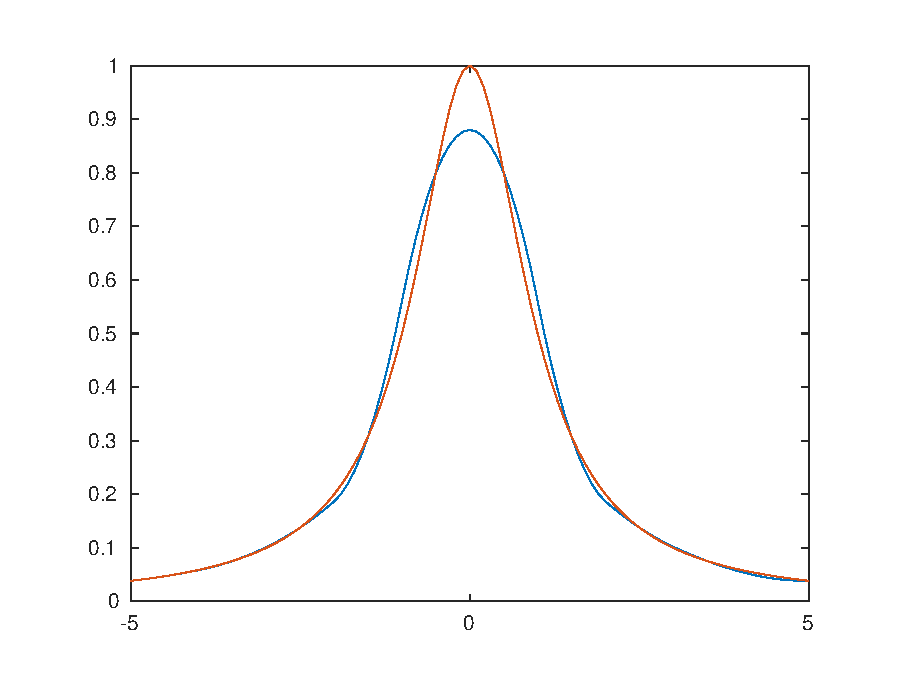
\includegraphics[width=6in]{./figure/quadratic_overall.eps}
\caption{overall quadratic B-spline}
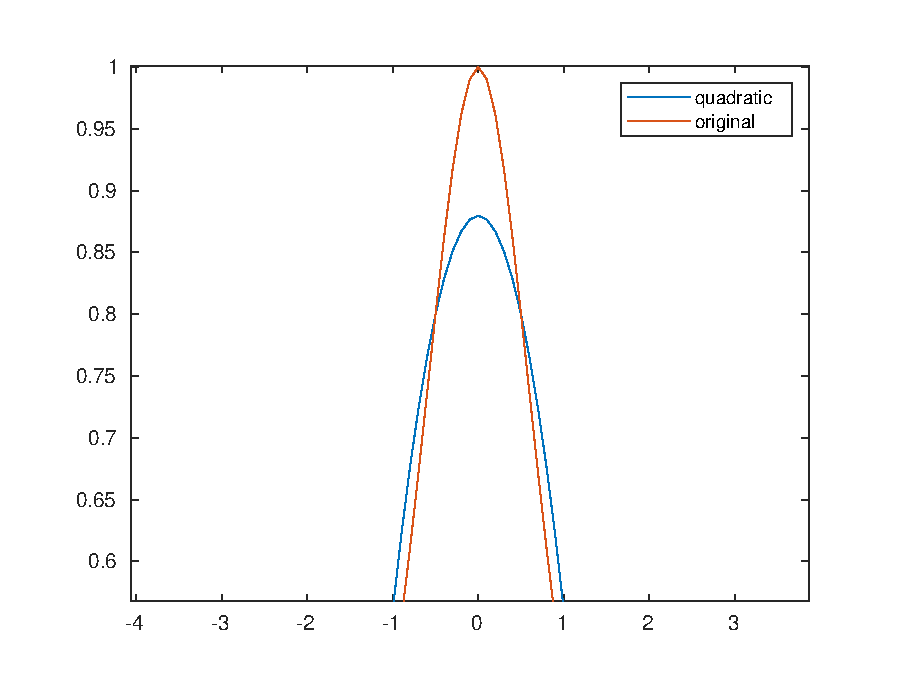
\includegraphics[width=6in]{./figure/quadratic_local.eps}
\caption{local quadratic B-spline}
\end{figure}
\begin{figure}[h]
\includegraphics[width=6in]{./figure/cubic_overall.eps}
\caption{overall quadratic B-spline}
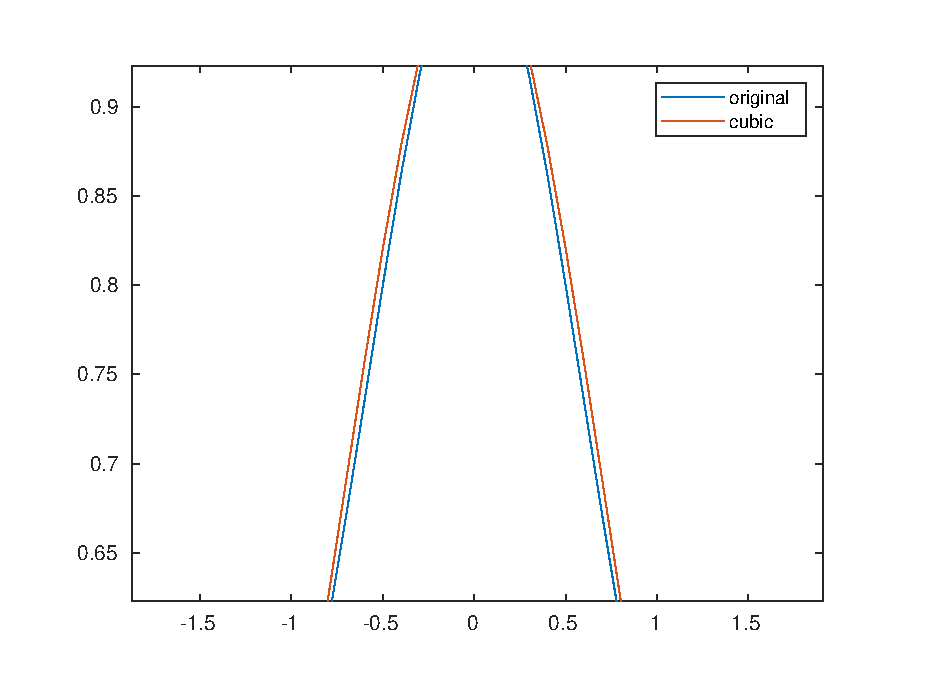
\includegraphics[width=6in]{./figure/cubic_local.eps}
\caption{local quadratic B-spline}
\end{figure}
\begin{figure}[h]
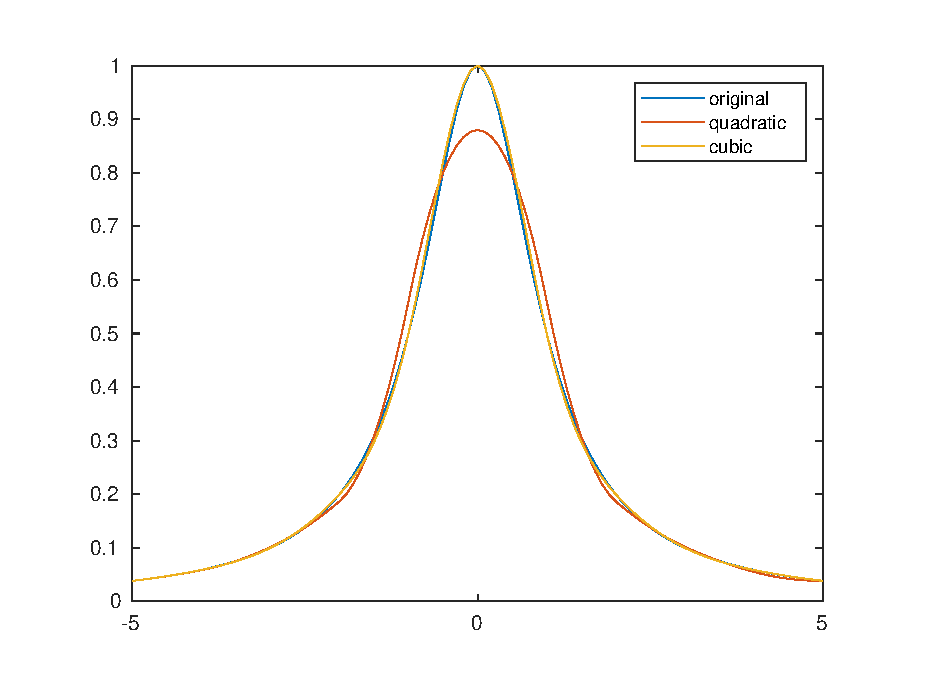
\includegraphics[width=6in]{./figure/qc_comp_overall.eps}
\caption{overall comparation}
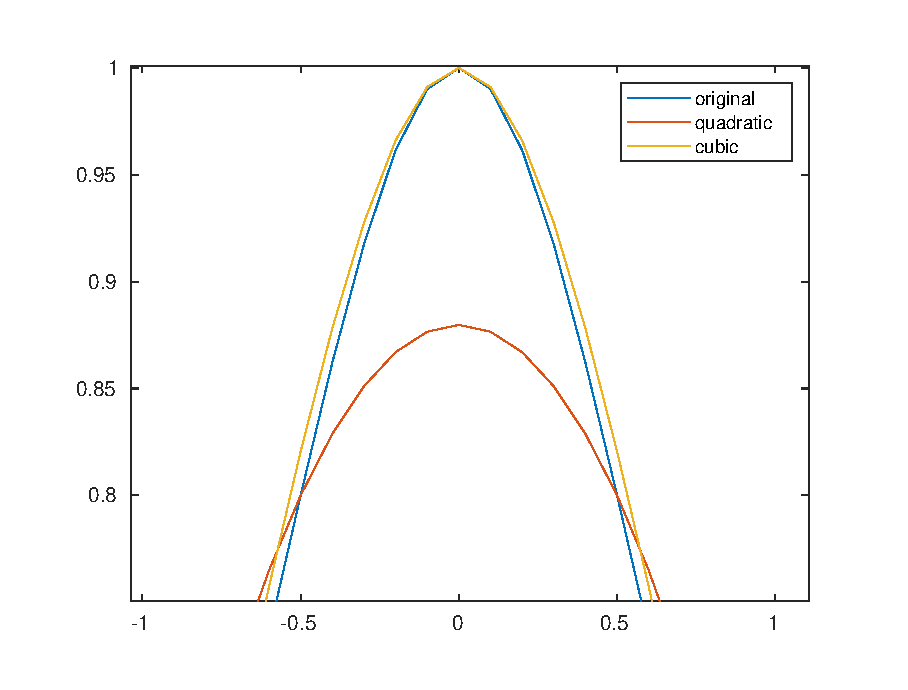
\includegraphics[width=6in]{./figure/qc_comp_local.eps}
\caption{local comparation}
\end{figure}

\subsection*{c.interpolation error}
\begin{tabular}{c|ccccccc}
quadratic&1.38778e-17 &0.0014184 &0 &0.120241 &1.11022e-16 &0.00197562 &0 \\
\hline
cubic &0.000669568 &0 &0.0205289 &1.11022e-16 &0.0205289 &0 &0.000669568 \\
\end{tabular}
\\
\\
As the chart shows that cubic interpolation is more close to the original function than quadratic interpolation overall, because the maximum of cubic interpolating errors is less than the quadratic. However, the quadratic is also precise near two end points. The some error are close to the machine procision because we use double to store numbers which occupies 64 bits. Error may come from the procedures solving the linear algebra problems and system abandons some overflowing bits. 

\subsection*{d.three plots of heart function}
Results are presented as Figure7 , Figure8 , Figure9.
\begin{figure}[h]
\includegraphics[width=6in]{./figure/n10.eps}
\caption{heart function for $n=10$}
\end{figure}

\begin{figure}[h]
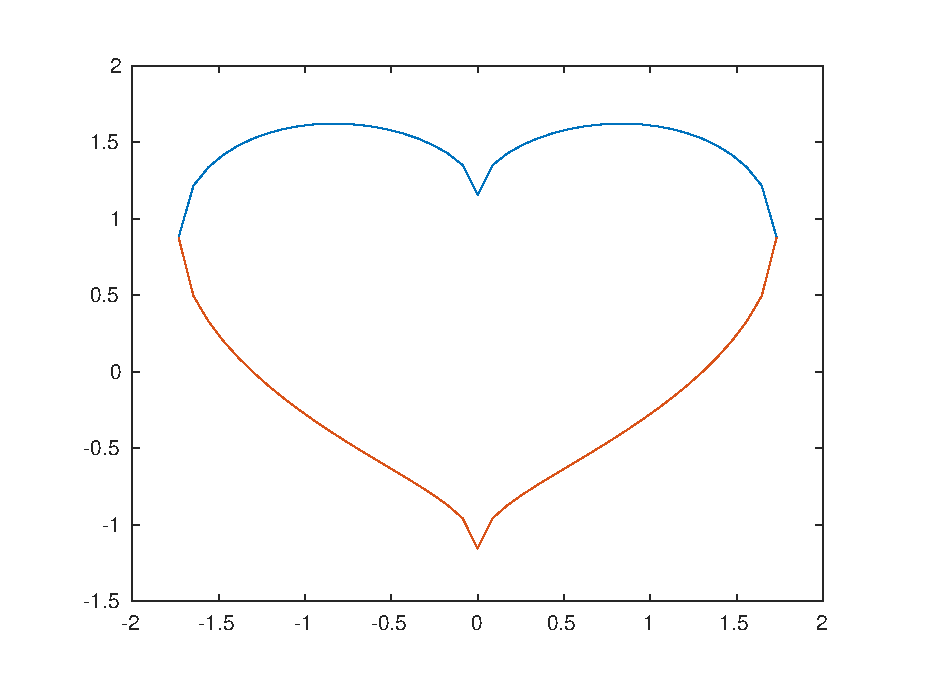
\includegraphics[width=6in]{./figure/n40.eps}
\caption{heart function for $n=40$}
\end{figure}

\begin{figure}[h]
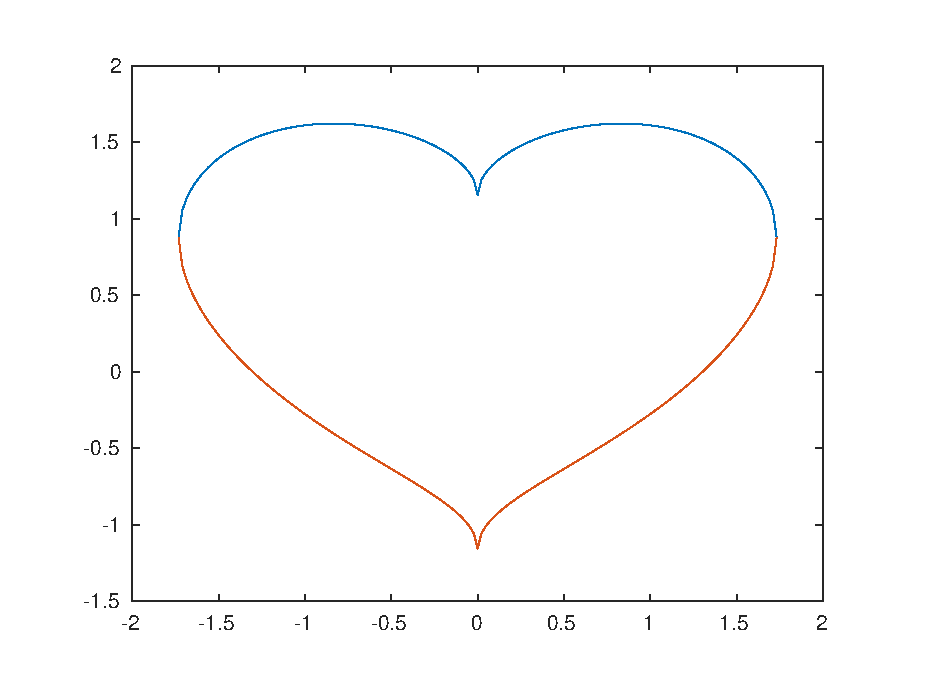
\includegraphics[width=6in]{./figure/n160.eps}
\caption{heart function for $n=160$}
\end{figure}
\end{document}

%%% Local Variables: 
%%% mode: latex
%%% TeX-master: t
%%% End: 
